%\documentclass[12pt, twoside]{book}
\documentclass[12pt, oneside]{book}  % jednostranna tlac

\let\cleardoublepage\clearpage

%spravne nastavenie okrajov
\usepackage[a4paper,top=2.5cm,bottom=2.5cm,left=3.5cm,right=2cm]{geometry}
%zapnutie fontov pre UTF8 kodovanie
\usepackage[utf8]{inputenc}
\usepackage[T1]{fontenc}

%nastavenie riadkovania podla smernice
\linespread{1.25} % hodnota 1.25 by mala zodpovedat 1.5 riadkovaniu

% balicek na vkladanie zdrojoveho kodu
\usepackage{listings}
\renewcommand{\lstlistingname}{Algorithm}
\lstset{frame=lines}

% balicek na vkladanie obrazkov
\usepackage{graphicx}
% balicek na vkladanie celych pdf dokumentov, tu zadanie
\usepackage{pdfpages}
% balicek na spravne formatovanie URL
\usepackage{url}
% balicek na hyperlinky v ramci dokumentu
\usepackage[hidelinks,breaklinks]{hyperref}

\setcounter{tocdepth}{3}   % show chapters, sections, subsections, subsubsections

% --- Pridane balicky pre tuto pracu ---
\usepackage{amsmath}          % matematicke prostredia a prikazy
\usepackage{amssymb}          % matematicke symboly (\checkmark atd.)
\usepackage{siunitx}          % SI jednotky: \SI{10}{\kilo\ohm}
\usepackage{longtable}        % tabulky presahujuce stranku
\usepackage{booktabs}         % profesionalne linky v tabulkach
% --- Koniec pridanych balickov ---

% Force a page break before a specific bibliography entry so its URL
% does not split across pages. Patches the internal \@lbibitem command
% (called by \bibitem[label]{key} as emitted by plain.bst).
\makeatletter
\let\orig@bibitem\@bibitem
\def\@bibitem#1{%
  \def\check@key{#1}\def\target@key{ref22}%
  \ifx\check@key\target@key
    \newpage
  \fi
  \orig@bibitem{#1}%
}
\makeatother

% -------------------
% --- Definicia zakladnych pojmov
% --- Vyplnte podla vasho zadania, rok ma byt rok odovzdania
% -------------------
\def\mfrok{2026}
\def\mfnazov{Hardware Design and Documentation of the UACS RFID Audio CAN Node}
\def\mftyp{Bachelor Thesis}
\def\mfautor{William Jozef Šimoňák}
\def\mfskolitel{Richard Ostertág}

%ak mate konzultanta, odkomentujte aj jeho meno na titulnom liste
%\def\mfkonzultant{tit. Meno Priezvisko, tit. }

\def\mfmiesto{Bratislava, \mfrok}

\def\mfodbor{Computer Science}
\def\program{Computer Science}

\def\mfpracovisko{Department of Computer Science}

\begin{document}
\frontmatter
\pagestyle{empty}

% -------------------
% --- Obalka ------
% -------------------

\begin{center}
  \sc\large
  Comenius University in Bratislava\\
  Faculty of Mathematics, Physics and Informatics

\vfill

{\LARGE\mfnazov}\\
\mftyp
\end{center}

\vfill

{\sc\large
\noindent \mfrok\\
\mfautor
}

\cleardoublepage
% --- koniec obalky ----

% -------------------
% --- Titulný list
% -------------------

\noindent

\begin{center}
\sc
\large
  Comenius University in Bratislava\\
  Faculty of Mathematics, Physics and Informatics

\vfill

{\LARGE\mfnazov}\\
\mftyp
\end{center}

\vfill

\noindent
\begin{tabular}{ll}
Study Programme: & \program \\
Field of Study:  & \mfodbor \\
Department:      & \mfpracovisko \\
Supervisor:      & \mfskolitel \\
% Consultant:    & \mfkonzultant \\
\end{tabular}

\vfill

\noindent \mfmiesto\\
\mfautor

\cleardoublepage
% --- Koniec titulnej strany


% -------------------
% --- Zadanie z AIS
% -------------------
\newpage
\setcounter{page}{3}
\hypersetup{pageanchor=false}
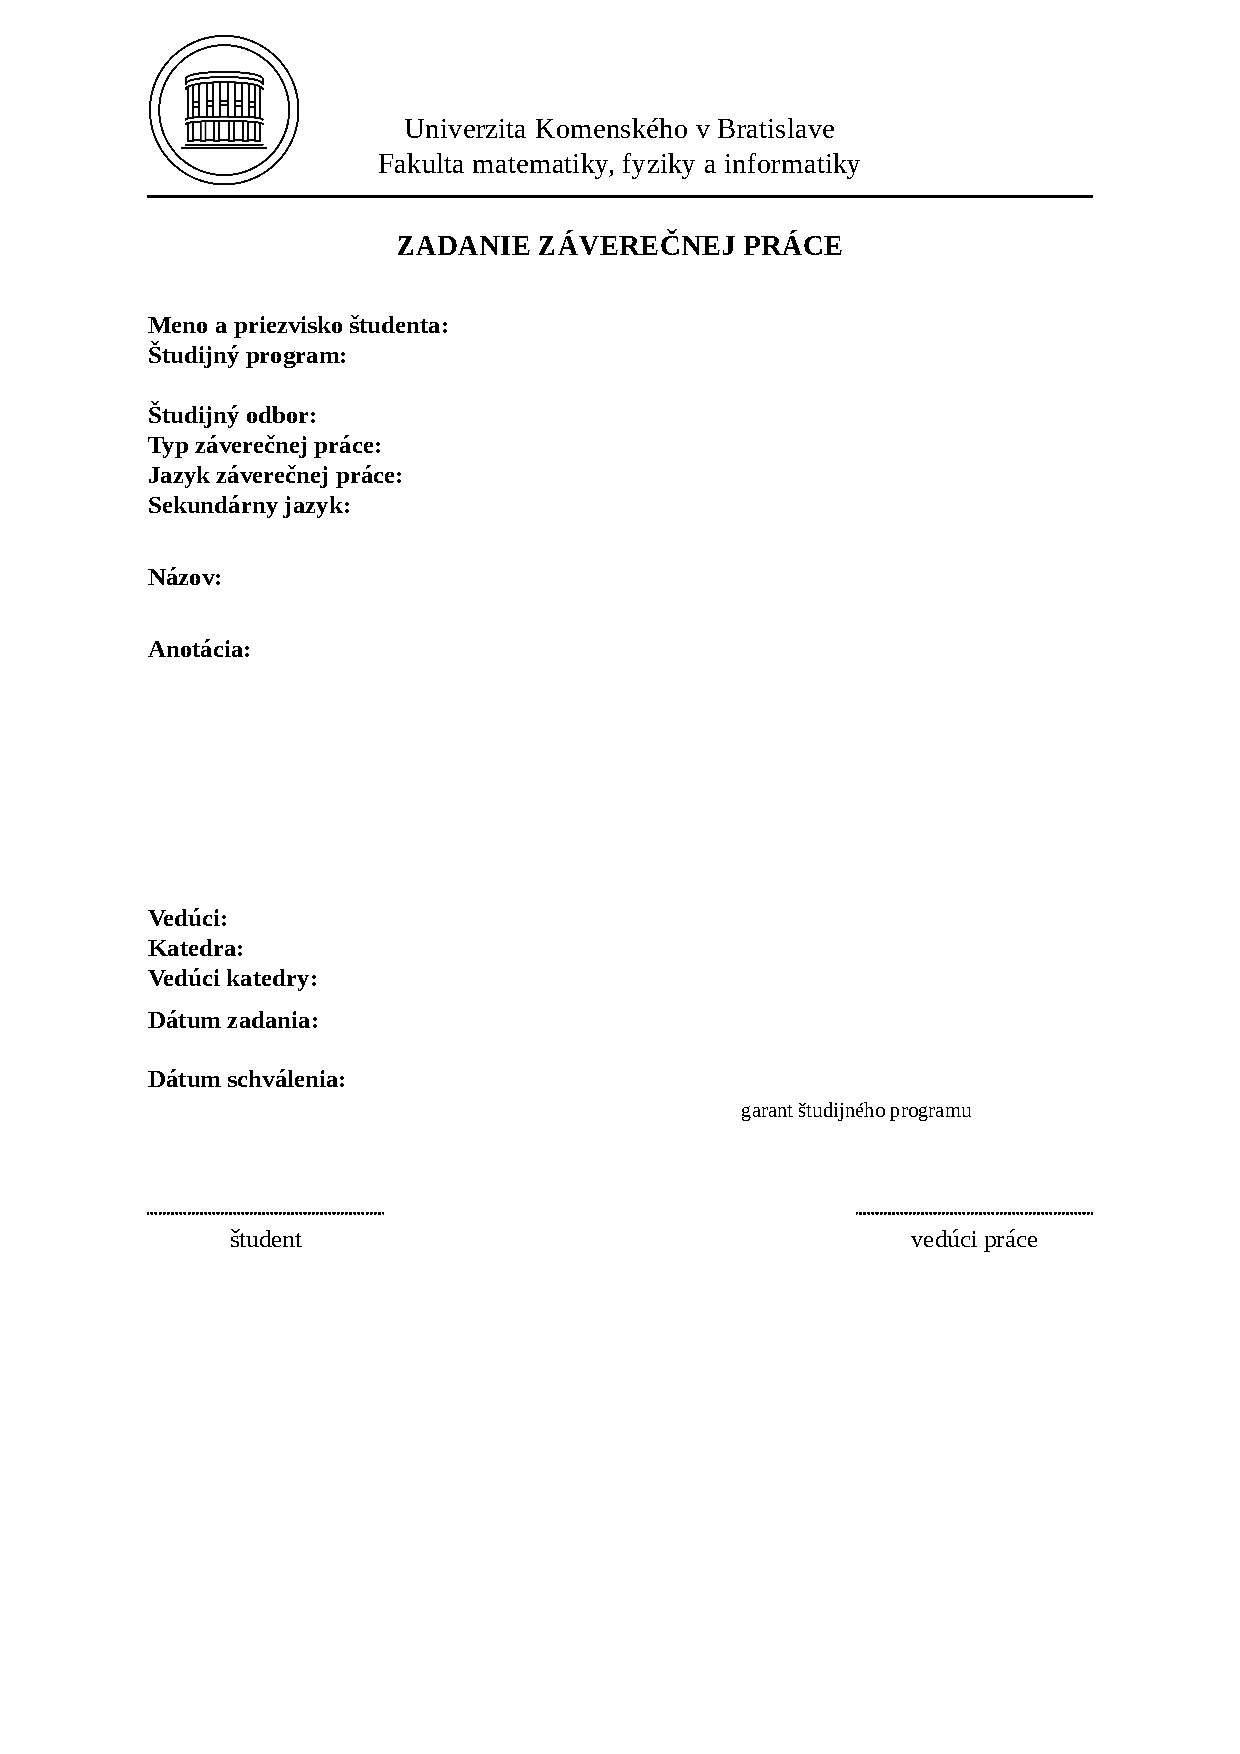
\includepdf{images/zadanie.pdf}
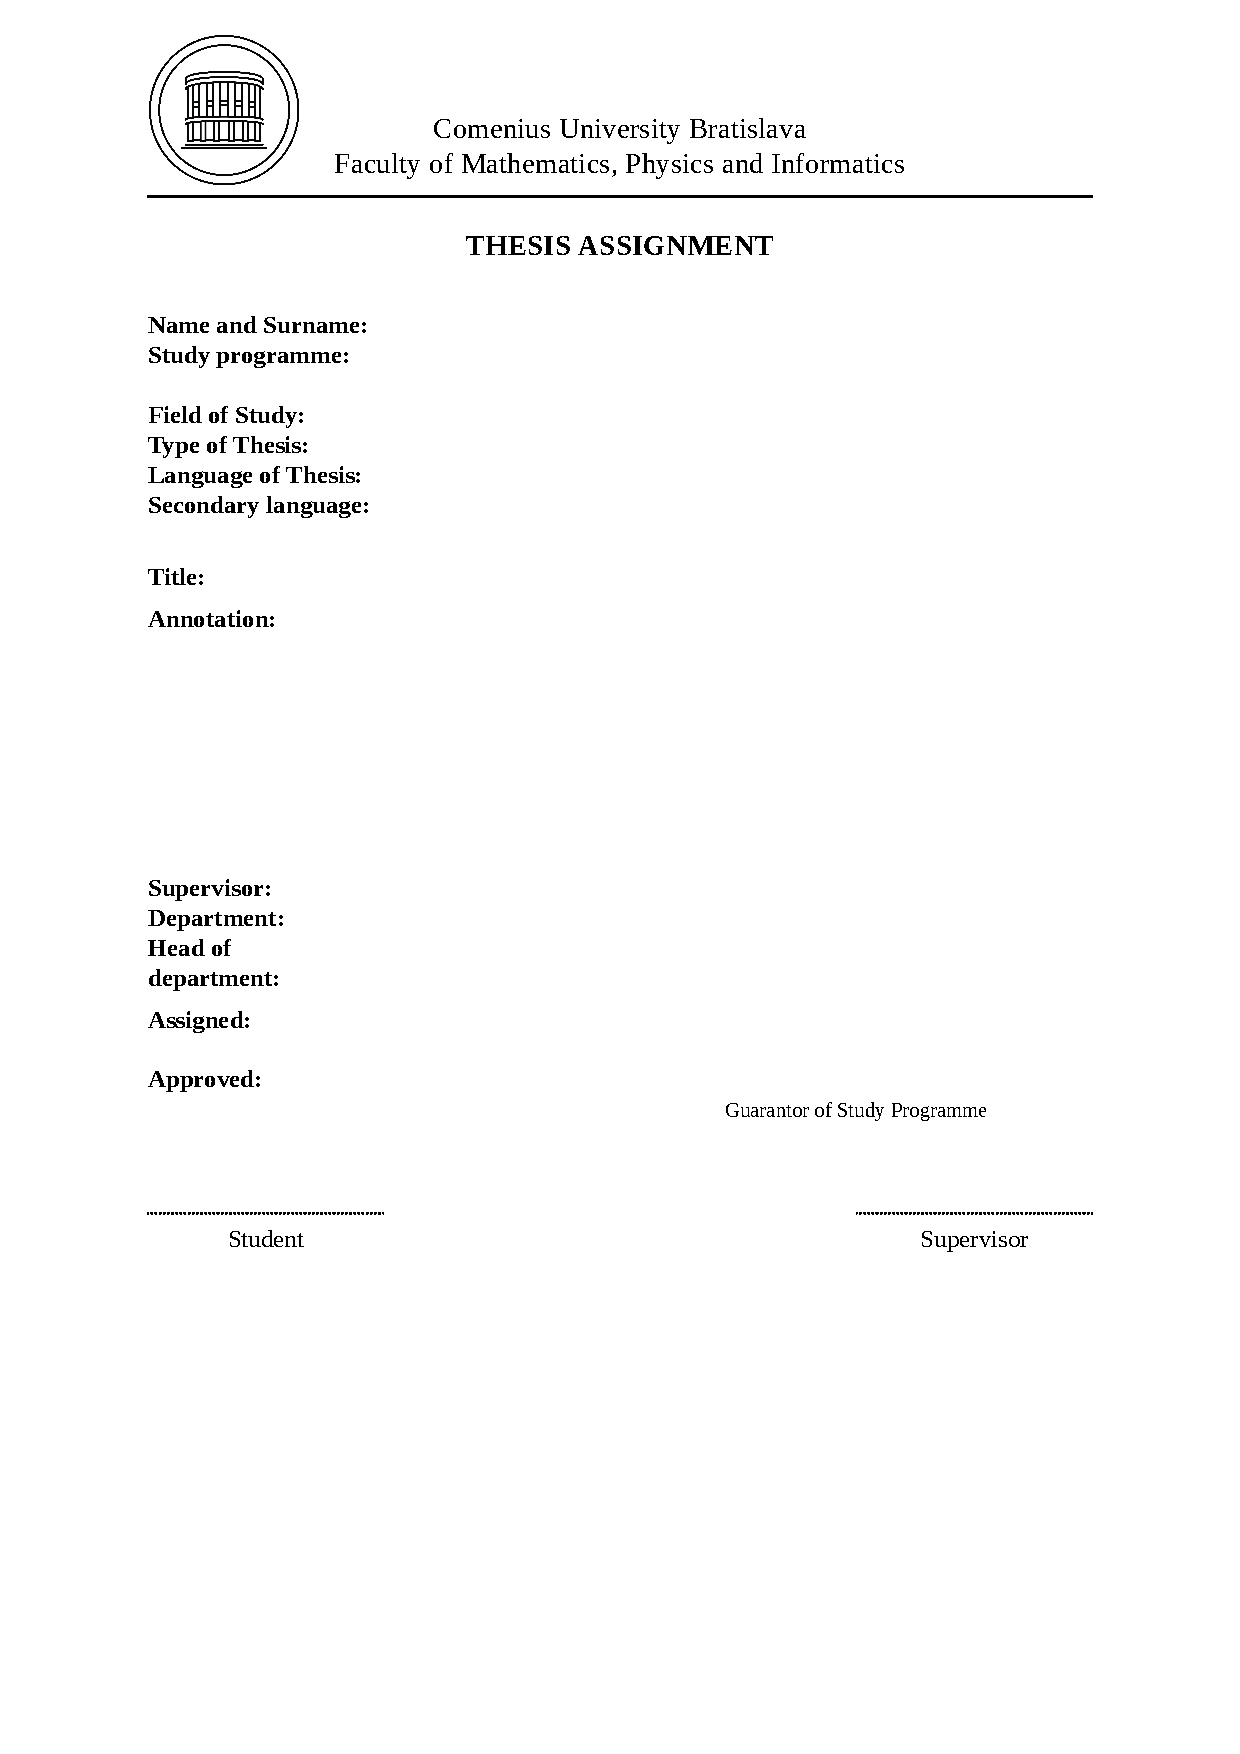
\includepdf{images/zadanie-en.pdf}
\hypersetup{pageanchor=true}
% --- Koniec zadania


% -------------------
%   Čestné vyhlásenie a nepovinné poďakovanie
% -------------------
\newpage
\pagestyle{plain}
\paragraph{Declaration:}
I hereby declare that I have independently written this entire
bachelor thesis entitled ``\mfnazov'', including all its
figures and appendices, using the literature listed in the attached
bibliography.

% Uveďte na čo ste nástroje používali
% Podľa typu použitia potom nástroje aj citujte v texte
In preparation of this thesis I have used the Claude AI assistant for the
following purposes: as a technical advisor on topics I was not previously
familiar with, for spelling and formatting corrections, for suggesting
sources I could use as a basis for claims, and for converting the thesis
from Markdown to \LaTeX{} format. I have used this tool in accordance with
relevant legal regulations, academic rights and freedoms, ethical and moral
principles while simultaneously maintaining academic integrity. I am aware
that I am fully responsible for the accuracy of the final text.

\paragraph{Acknowledgments:}
% TODO: Poďakovanie školiteľovi a ďalším osobám

% --- Koniec poďakovania

% -------------------
%   Abstrakt - Slovensky
% -------------------
\newpage
\section*{Abstrakt}


\paragraph*{Kľúčové slová:} UACS, RFID, CAN FD, STM32H523, doska plošných spojov, hardvérový návrh
% --- Koniec Abstrakt - Slovensky


% -------------------
% --- Abstrakt - Anglicky
% -------------------
\newpage
\section*{Abstract}


\paragraph*{Keywords:} UACS, RFID, CAN~FD, STM32H523, printed circuit board, hardware design

% --- Koniec Abstrakt - Anglicky


% -------------------
% --- Obsah
% -------------------

\cleardoublepage

\tableofcontents

% ---  Koniec Obsahu

% -------------------
% --- Zoznamy tabuliek, obrázkov
% -------------------

\newpage

\listoffigures
\listoftables

% ---  Koniec Zoznamov

\mainmatter
\pagestyle{plain}

\input intro.tex

\input chapter1.tex

\addtocontents{toc}{\protect\clearpage}
\input appendixA-en.tex

\input chapter2.tex

\input conclusion.tex


% -------------------
% --- Bibliografia
% -------------------

\newpage

\backmatter

\thispagestyle{empty}
\clearpage
\addcontentsline{toc}{chapter}{References}
\bibliographystyle{plain}
\bibliography{literatura}

%---koniec Referencii

\end{document}
